\section{User-Friendly Knowledge Graph Construction Approaches \textcolor{shamrockgreen}{-- Done!}}
\label{sec:chp2_easy_kgc}

This section presents the different approaches developed for easing the writing of mapping rules for practitioners. We divide these approaches into two categories, (i) visual editors (\cref{sec:chp2_visual-editors}) that rely in an interactive application to graphically depict and edit mappings, and (ii) serializations (\cref{sec:chp2_serializations}) that rely on a simplified syntax for writing the mapping rules. \cref{tab:chp2_easy-mappings} lists the approaches described in the remaining of the section.

\begin{table}[t]
\caption[Approaches for easy mapping creation]{Approaches for facilitating the mapping creation process for users. The proposals are divided into (i) visual editors and (ii) text-based serializations. For each proposal, the reference, compliant mapping language and subtype is provided.}
\label{tab:chp2_easy-mappings}
\resizebox{\columnwidth}{!}{
\centering
\begin{tabular}{cccc}
%\rowcolor[HTML]{EFEFEF} 
\textbf{Classification} & \textbf{Approach} & \textbf{Mapping Language} & \textbf{Type} \\ \midrule
\multirow{15}{*}{\textbf{Visual Editor}} & ODEMapster~\parencite{barrasa2006odemapster} & R2O & Tree \\
 & Karma~\parencite{gupta2012karma} & R2RML & Tree \\
 & RBA~\parencite{neto2013rba} & R2RML & Tree \\
 & \cite{sengupta2013editing} & R2RML & Building blocks \\
 & \cite{lembo2014visualization} & R2RML & Graph \\
 & RMLEditor~\parencite{heyvaert2016rmleditor} & R2RML/RML & Graph \\
 & SQuaRE~\parencite{blinkiewicz2016square} & R2RML & Graph \\
 & OntopPro~\parencite{calvanese2017ontop} & Proprietary & Building blocks \\
 & Juma~\parencite{junior2017juma} & R2RML & Building blocks \\
 & RMLx~\parencite{aryan2017rmlx} & RML & Building blocks \\
 & Map-On~\parencite{sicilia2017map} & R2RML & Graph \\
 & gra.fo\tablefootnote{\label{foot:gra.fo}\url{https://gra.fo/}} & R2RML & Graph \\
 & Stardog designer\tablefootnote{\label{foot:stardog-designer}\url{https://www.stardog.com/designer/}} & SMS2 & Graph \\
 & Ontopic Studio\tablefootnote{\label{foot:ontopic-studio}\url{https://ontopic.ai/en/ontopic-studio/}} & R2RML/Proprietary & Building blocks \\
 & Eccenca Corporate Memory\tablefootnote{\label{foot:eccenca}\url{https://documentation.eccenca.com/latest/build/lift-data-from-tabular-data-such-as-csv-xslx-or-database-tables}} & Proprietary & Building blocks \\ \midrule
\multirow{5}{*}{\textbf{Serialization}} & SML~\parencite{Stadler2015sml} & R2RML & SPARQL-based \\
 & Ontop proprietary~\parencite{calvanese2017ontop} & R2RML & TTL- and SQL-based \\
 & YARRRML~\parencite{Heyvaert2018yarrrml} & RML & YAML-based \\
 & SMS2\tablefootnote{\label{foot:sms2}\url{https://docs.stardog.com/archive/7.5.0/virtual-graphs/mapping-data-sources.html\#sms2-stardog-mapping-syntax-2}} & R2RML & SPARQL-based \\
 & XRM\tablefootnote{\label{foot:xrm}\url{https://zazuko.com/products/expressive-rdf-mapper/}} & R2RML/RML/CSVW & Proprietary syntax \\ \bottomrule
\end{tabular}
}
\end{table}

\subsection{Visual Editors}
\label{sec:chp2_visual-editors}

Visual editors were first developed for enhancing and easing the mapping writing process. We can subdivide the proposals released over the years based on how the mapping is graphically represented in the tool: either with a tree or graph layout, or using building blocks (\cref{fig:chp2_visual-editors}).


\begin{figure*}[t]
\centering
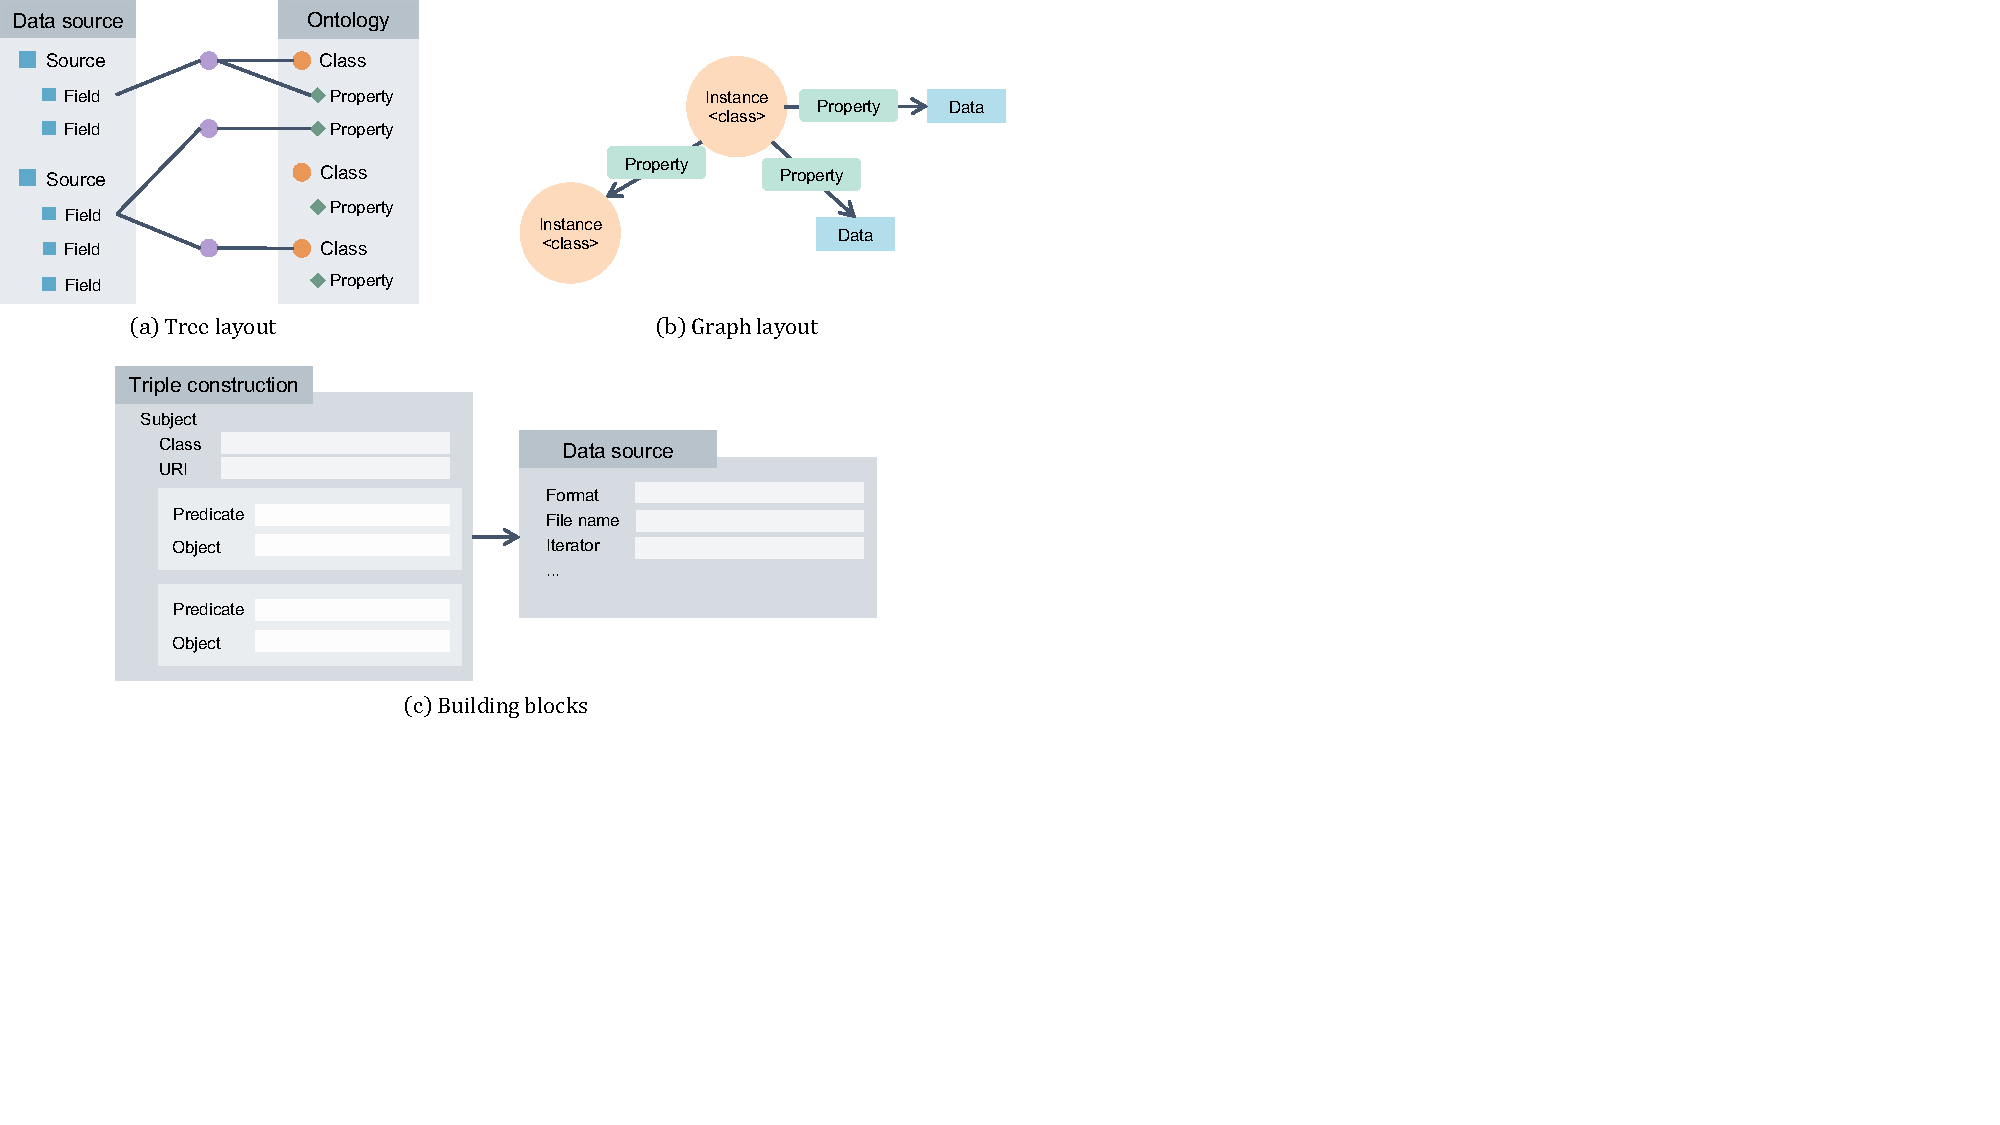
\includegraphics[width=0.9\linewidth]{figures/chp2_visual-editors.pdf}
\caption[Graphical representations approaches in visual mapping editors.]{Graphical representations approaches in visual mapping editors: (a) tree layout, (b) graph layout, and (c) building blocks.}
\label{fig:chp2_visual-editors}
\end{figure*}

The tree layout succeeded in the first approaches developed. 
The first one was developed for the R$_2$O mapping language in ODEMapster~\parencite{barrasa2006odemapster}, providing a graphical interface to visualize and edit the mappings by link the database elements with the ontology resources. 
After the release of R2RML, Karma~\parencite{gupta2012karma} and RBA (R2RML by assertion)~\parencite{neto2013rba} were developed for this language. Both work similarly to ODEMapster, with the addition of Karma providing automatic mapping suggestions. 

The graph display was later adopted by multiple editors, such as in \cite{lembo2014visualization}, SQuaRE~\parencite{blinkiewicz2016square}, RMLEditor~\parencite{heyvaert2016rmleditor} and Map-On~\parencite{sicilia2017map}. These editors provide a graph overview of the mapping while constructing it, while also showing the data sources and ontology. All of them are able to create R2RML mappings, and in addition, the RMLEditor can also produce RML mappings. There are also non open-source editors developed by companies that use a graph layout, such as \url{gra.fo}\cref{foot:gra.fo} and the Stardog designer\cref{foot:stardog-designer}. The former works with R2RML, and the latter with the Stardog proprietary syntax, SMS2, described in the next section. 

%~\parencite{fu2013tree-vs-graph} 

Some tools were also developed that follow an alternative approach to the tree and graph layouts, broadly used in the semantic web supporting applications. This approach comprises the use of building blocks or templates, that are the components to build a mapping between data source and ontology. The first editor following this approach was proposed in \cite{sengupta2013editing}, later refined in \cite{pinkel2014best}. OntopPro~\parencite{calvanese2017ontop} released a Protégé plugin to create and edit mappings (in their proprietary language) with templates, allowing also the creation of RDF triples and running SPARQL queries. Juma~\parencite{junior2017juma} and RMLx~\parencite{aryan2017rmlx} allow building R2RML and RML mappings respectively with building blocks, correspondent to the different parts of the mappings. There are also a couple of examples that enable this kind of visualization for mapping construction but using a proprietary language, Ontopic Studio\cref{foot:ontopic-studio} and Eccenca Corporate Memory\cref{foot:eccenca}. 



\subsection{Serializations}
\label{sec:chp2_serializations}

As an alternative to visual approaches, text-based user-friendly serializations were developed. This approach suited most practitioners with technical profiles or with preferences for a text oriented environment. 
SML~\parencite{Stadler2015sml} was developed as user-friendly syntax for R2RML. It provides an SPARQL-based syntax, enhancing the simplicity for writing mappings but maintaining the same expressiveness. 
The virtual KG processor Ontop~\parencite{calvanese2017ontop} also provides a simplified serialization for R2RML, which combines the Turtle syntax for triple generation and SQL for data access. 
The Stardog triplestore developed another SPARQL-based proprietary serialization, the Stardog Mapping Syntax 2 (SMS2)\cref{foot:sms2}. 

Later on, as more mapping languages emerged, new serializations with a broader language range emerged. This is the case of XRM\cref{foot:xrm} (Expressive RDF Mapper), that provides a unique syntax for writing R2RML, RML and CSVW mappings. It can be used with a service plugin integrated into common text editors, Visual Studio Code and Eclipse. This service warns the users about writing errors while writing, and translates the mapping rules into one of the aforementioned languages. 

YARRRML~\parencite{Heyvaert2018yarrrml}, the YAML-based\footnote{\url{https://yaml.org/spec/1.2.2/}} user-friendly syntax created for RML. 
\cref{lst:chp2_yarrrml-mapping} shows an example of a YARRRML mapping equivalent to the RML example shown in \cref{lst:chp2_rml-mapping}. 
YARRRML mappings need as well the declaration of the prefixes at the beginning of the document, which is done using the \texttt{prefixes} key (Lines 1-2). The mapping rules are defined within the \texttt{mappings} key (Lines 4-13), which are aggregated in rule set with keys named by the user (e.g. \texttt{athletes} key, Line 5). Each mapping rule set describes the input data sources (\texttt{sources} key, Lines 6-7), subject (\texttt{s} key, Line 8) and predicate-object pairs (\texttt{po} key, Lines 9-11).
This serialization can be used with the Matey\footnote{\url{https://rml.io/yarrrml/matey/}}, a web service able to translate YARRRML into RML mapping files, or directly generate RDF triples. 

\begin{captionedlisting}{lst:chp2_yarrrml-mapping}{YARRRML mapping to generate the RDF graph in \cref{lst:chp2_r2rml-result-rdf} with data from the JSON file shown in \cref{lst:chp2_json-example}. This mapping translates into the RML mapping shown in \cref{lst:chp2_yarrrml-mapping}.}
\centering
{\begin{lstlisting}[language=yarrrml]
prefixes:
 ex: "http://example.com/ns#"

mappings:
  athletes:
    sources:
      - ["data.json~jsonpath", "$\dollar$.*"]
    s: http://example.com/athlete/$\dollar$(RANK)
    po:
      - [a, ex:Athlete]
      - [ex:name, $\dollar$(NAME)]
      - [ex:rank, $\dollar$(RANK)]
      - [ex:mark, $\dollar$(MARK)]
\end{lstlisting}}
\end{captionedlisting}
